\documentclass[a4paper]{arrowhead}

\usepackage[yyyymmdd]{datetime}
\usepackage{etoolbox}
\usepackage[utf8]{inputenc}
\usepackage{multirow}

\renewcommand{\dateseparator}{-}

%% Special references
\newcommand{\mref}[1]{{\textcolor{ArrowheadPurple}{\hyperref[sec:model:#1]{#1}}}}
\newcommand{\oref}[1]{{\textcolor{ArrowheadBlue}{\hyperref[sec:operations:#1]{#1}}}}
\newcommand{\pdef}[1]{{\textcolor{ArrowheadGrey}{#1\label{sec:model:primitives:#1}
      \label{sec:model:primitives:#1s}\label{sec:model:primitives:#1es}}}}
\newcommand{\pref}[1]{{\textcolor{ArrowheadGrey}{\hyperref[sec:model:primitives:#1]{#1}}}}

\newrobustcmd\osubsection[3]{
  \addtocounter{subsection}{1}
  \addcontentsline{toc}{subsection}{\protect\numberline{\thesubsection}Interface
    operation \textcolor{ArrowheadBlue}{#1}}
  \renewcommand*{\do}[1]{\rref{##1},\ }
  \subsection*{
    \thesubsection\quad
    Interface operation
    \textcolor{ArrowheadBlue}{#1}
    (\notblank{#2}{\mref{#2}}{})
    \notblank{#3}{: \mref{#3}}{}
  }
  \label{sec:operations:#1}
}
\newrobustcmd\msubsection[2]{
  \addtocounter{subsection}{1}
  \addcontentsline{toc}{subsection}{\protect\numberline{\thesubsection}#1 \textcolor{ArrowheadPurple}{#2}}
  \subsection*{\thesubsection\quad#1 \textcolor{ArrowheadPurple}{#2}}
  \label{sec:model:#2} \label{sec:model:#2s} \label{sec:model:#2es}
}
%%

\begin{document}

%% Arrowhead Document Properties
\ArrowheadTitle{Monitoring} % XXX = ServiceName 
\ArrowheadServiceID{ID} % ID name of service
\ArrowheadType{Service Description}
\ArrowheadTypeShort{SD}
\ArrowheadVersion{5.0.0} % Arrowhead version X.Y.Z, e..g. 4.4.1
\ArrowheadDate{\today}
\ArrowheadAuthor{Jerker Delsing} % Corresponding author e.g. Jerker Delsing
\ArrowheadStatus{PROTOTYPE} % e..g. RELEASE, RELEASE CONDIDATE, PROTOTYPE
\ArrowheadContact{jerker.delsing@ltu.se} % Email of corresponding author
\ArrowheadFooter{\href{www.arrowhead.eu}{www.arrowhead.eu}}
\ArrowheadSetup
%%

%% Front Page
\begin{center}
  \vspace*{1cm}
  \huge{\arrowtitle}

  \vspace*{0.2cm}
  \LARGE{\arrowtype}
  \vspace*{1cm}

  %\Large{Service ID: \textit{"\arrowid"}}
  \vspace*{\fill}

  % Front Page Image
  %\includegraphics{figures/TODO}

  \vspace*{1cm}
  \vspace*{\fill}

  % Front Page Abstract
  \begin{abstract}
    Monitoring of any microsystem and its produced and consumed
    microservices is important in a professional indutrial
    context. The Monitoring service provides some very basic interface key-pairs
    and a possibility to for dynamically update it self with modified, new
    or even removed interface key-pairs. All key-pairs are
    necessitated to be provided as meta-data to the service registration. 
  \end{abstract}

  \vspace*{1cm}

%   \scriptsize
%   \begin{tabularx}{\textwidth}{l X}
%     \raisebox{-0.5\height}{
\includegraphics[width=2cm]{figures/artemis_logo}} & {ARTEMIS Innovation Pilot Project: Arrowhead\newline
%     THEME [SP1-JTI-ARTEMIS-2012-AIPP4 SP1-JTI-ARTEMIS-2012-AIPP6]\newline
%     [Production and Energy System Automation Intelligent-Built environment and urban infrastructure for sustainable and friendly cities]}
%   \end{tabularx}
%   \vspace*{-0.2cm}
 \end{center}

\newpage
%%

%% Table of Contents
\tableofcontents
\newpage
%%

\section{Overview}
\label{sec:overview}

This document describes the Monitoring service, which enables very
basic basic monitoring of a microsystem and its micrcoservices. 
The Monitoring service provides one very basic interface
    and mechanisms for dynamically update it self with modified, new
    or even removed interfaces.

The rest of this document is organized as follows.
In Section \ref{sec:operations}, we describe the abstract message
operations provided by the service.
In Section \ref{sec:model}, we end the document by presenting the data types used by the mentioned operations.

%\newpage

\subsection{Significant Prior Art}

Monitoring is not a simple service. For Arrowhead v4.6 and earlier
individual services may have an echo interface.

\subsection{How This Service Is Meant to Be Used}

The monitoring service is a mandatory service for all core and support
microsystems and a highly recomended service for any application
microsystem.

The general idea is that a Monitor microsystem subscribes to all
avialable Monitoring service. The subscription can hold conditions
like e.g. time interval, battery level below X\%, error reports.

The usage scenario is depicted in Figure \ref{fig:Monitoring}

\begin{figure}[h!]
  \centering
  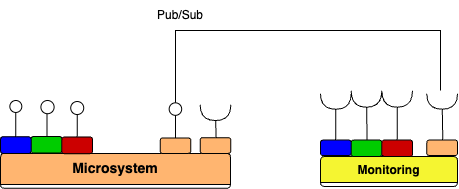
\includegraphics[width=10cm]{figures/Monitor_architecture}
  \caption{The general architectural usage of the Monitoring service isSysML SD diagram of the Monitoring service and its basic interfaces}
  \label{fig:Monitoring}
\end{figure}


This service is intended to provides the capability to monitor status of a
microsystem and its associated microservices. Example of statuses are:
\begin{itemize}
\item Echo alive
\item Power monitoring
\item Test consumption of service for which the microsystem has a
  consumer.
\item Internal state of the microsystem, e.g. remaining
  usefull life, ....
\item Trigger a subscription push of data to a consumer
\item Update of the monitoring service
\end{itemize}





\subsection{Important Delimitations and Dependencies}
\label{sec:delimitations}

The service privides only a very limited basic monitoring interfaces.
Dynamically the servcie can be modified with updated, new or rewoked interfaces. 
A specifc upddate interface will be provided. This one can be
protected nad thus limited to only accept systems or user comsumptions
with certain certificate level. Specific security concerns need to be
addressed while using this Update interface. 

%\newpage

\section{Service Interface}
\label{sec:operations}


The Monitoring service has the interface depicted in \ref{fig:SD}

\begin{figure}[h!]
  \centering
  \includegraphics[width=10cm]{figures/Monitor\_SD}
  \caption{SysML SD diagram of the Monitoring service and its basic interfaces}
  \label{fig:SD}
\end{figure}

The following basic interfaces are available.


\osubsection{Echo}{Pull/Push,XXh}{StatusCode,StatusCodeKind}

The Echo interface will responde with an TCP responde code
e.g. 100. Thus indicateing things are working as expected.
The Echo interface shoul be possible to subscribe to or make a pull request.
For the subscription an alive update will be pushed every XX
hour. Default XX is 24 hours.

\osubsection{Power}{type,level}{type, level}

The Power interface input parameters are: type and level.
Type=line|battery|harvesting
Level= XX\% (subscription to power level going below xx\% and repeated
alert every 5\% reduction in supply level) 

The responses are:
Type=line|battery|harvesting
Level=x[V]|xx\%|nn[A] dependent on the Type value.


\osubsection{AdditionalMonitoringTypel}{X,Y}{A,B}
Additional interfaces can be added by the individual producing
microsystem. This is done specifiying
\begin{itemize}
  
\item interface: MonitoringType, e.g. FreeMemory
\item RequestParameters, e.g. MemoryType : FreeMemValue
\item ResponseParameters, e.g. DRAM : 2kB
\end{itemize}  

Additional interfaces data need to be provided as metadata to the ServiceRegistry when
registering using the ServiceDiscovery service.  

%\newpage

\section{Information Model}
\label{sec:model}

% \color{red} 
% Here, all data objects that can be part something the XX Service
% provides to the hosting System are listed in alphabetic order.
% Note that each subsection, which describes one type of object, begins with the \textit{struct} keyword, which is used to denote a collection of named fields, each with its own data type.
% As a complement to the explicitly defined types in this section, there is also a list of implicit primitive types in Section \ref{sec:model:primitives}, which are used to represent things like hashes and identifiers.

% EXAMPLE data object types are illustrated in Figure \ref{fig:model_overview}.

% \color{black}

% \begin{figure}[ht!]
%   \centering
%   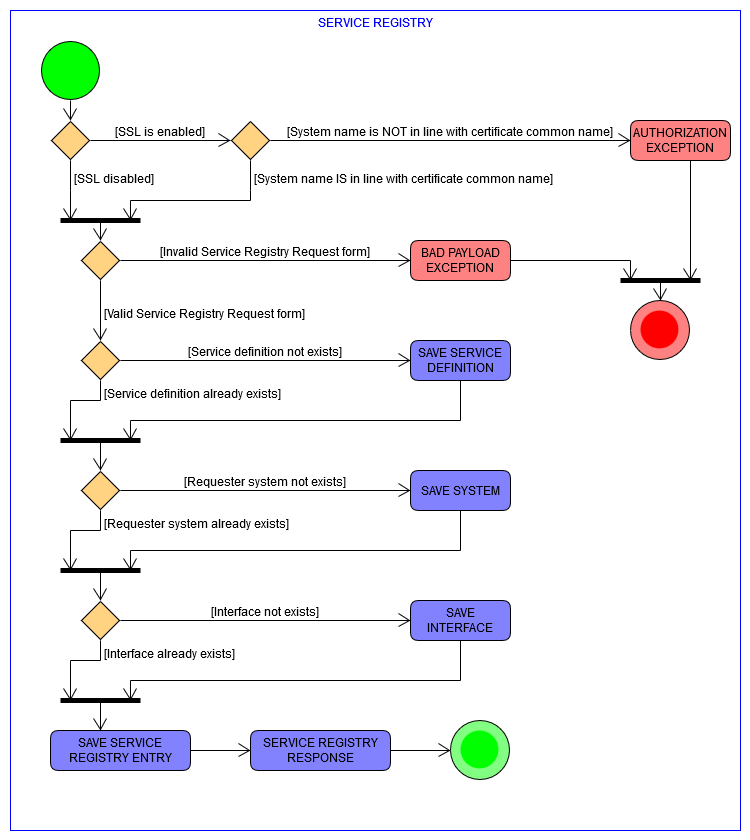
\includegraphics[width=\textwidth]{figures/post_service_registry_register_activity_uml}
%   \caption{\color{red} EXAMPLE:
%     Information model as a UML activity diagram.
%     Describes the process of service registration.
%     \color{black}
%   }
%   \label{fig:model_overview}
% \end{figure}

\msubsection{struct}{-,-}{echo,alive}

This structure is used to get an echo from the Monitor service
based on StatuCodeKind.
 
% \begin{table}[ht!]
% \begin{tabularx}{\textwidth}{| p{4.25cm} | p{3.5cm} | X |} \hline
% \rowcolor{gray!33} Field & Type      & Description \\ \hline
% endofValidity                 & \pref{DateTime} & Service is available until this UTC timestamp. \\ \hline
% interfaces                   & \pref{Array}$<$\pref{Interface}$>$     & List of interfaces the service supports. \\ \hline
% metadata                  & \pref{Metadata}     & Metadata \\ \hline
% providerSystem                    & \pref{Name} & Name of the provider system. \\ \hline
% secure                   &\pref{SecureType}  & Type of security the service uses. \\ \hline
% serviceDefinition         &\pref{Name}        & Service Definition. \\ \hline
% serviceUri                &\pref{URI}         & URI of the service. \\ \hline
% version                   &\pref{Version}     & Version of the service. \\ \hline
% \end{tabularx}
% \end{table}

% \begin{figure}[ht!]
%   \centering
%   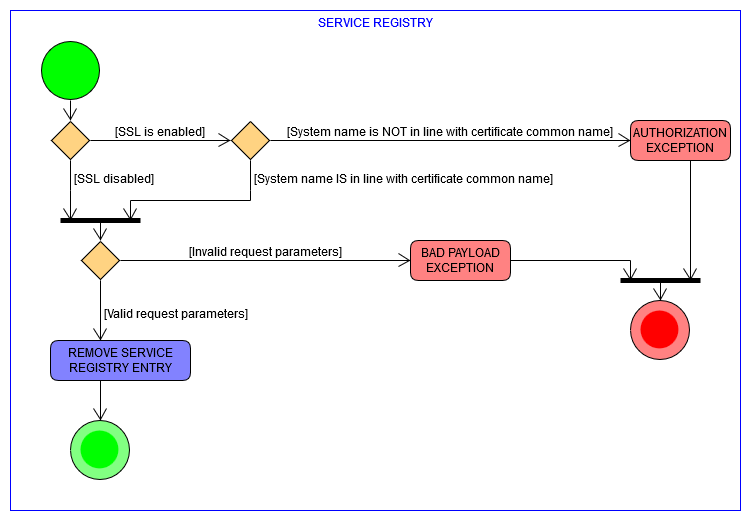
\includegraphics[width=\textwidth]{figures/delete_service_registry_unregister_activity_uml.png}
%   \caption{\color{red}  EXAMPLE:
%     Information model as a UML activity diagram.
%     Describes the process of service unregistration.
%     \color{black}
%   }
%   \label{fig:unregister_overview}
% \end{figure}

\msubsection{struct}{power, level}

Provide type of power supply e.g. line, battery, harvesting.
Provides level of power e.g. \%, energy


% EXAMPLE: This structure is used to register a service offering into
% the Service Registry. Please also refer to the activity diagram in
% Figure \ref{fig:unregister_overview} \color{black}

% \begin{table}[ht!]
% \begin{tabularx}{\textwidth}{| p{4.25cm} | p{3.5cm} | X |} \hline
% \rowcolor{gray!33} Field & Type      & Description \\ \hline
% address                 & \pref{Address} & Address of the provider systems. \\ \hline
% port                   & \pref{PortNumber}     & Port of the provider system. \\ \hline
% system\_name                  & \pref{Name}     & System name of the provider system \\ \hline
% service\_definition                    & \pref{Name} & Service Definition of the unregistered service. \\ \hline
% \end{tabularx}
% \end{table}

% \begin{figure}[ht!]
%   \centering
%   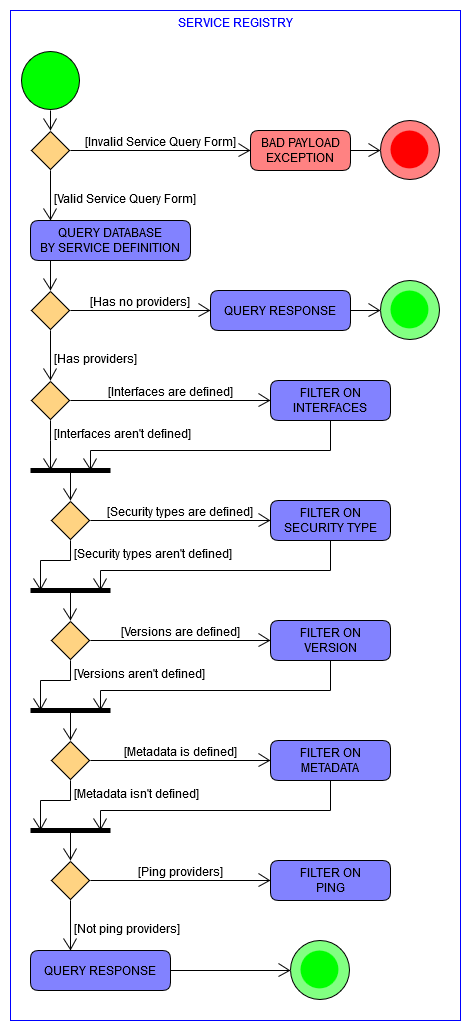
\includegraphics[width=\textwidth,height=0.9\textheight,keepaspectratio]{figures/post_service_registry_query_activity_uml.png}
%   \caption{\color{red}  EXAMPLE:
%     Information model as a UML activity diagram. Describes the process
%     of service querying.
%     \color{black}
%   }
%   \label{fig:query_overview}
% \end{figure}


\color{red} 

\msubsection{struct}{CC}

EXAMPLE: This structure is used to query service offering registered in
the Service Registry. Please also refer to the activity diagram in
Figure \ref{fig:query_overview} \color{black}

% \begin{table}[ht!]
% \begin{tabularx}{\textwidth}{| p{5cm} | p{3.5cm} | X |} \hline
% \rowcolor{gray!33} Object Field & Value Type      & Description \\ \hline
% "interfaceRequirements"                   & \pref{Array}$<$\pref{Interface}$>$     & List of the required interfaces. \\ \hline
% "maxVersionRequirement"                & \pref{Version}     & Maximum version. \\ \hline
% "minVersionRequirement"                & \pref{Version}     & Minimum version. \\ \hline
% "metadataRequirements"                  & \pref{Metadata}     & Metadata. \\ \hline
% "pingProviders".                    & \pref{Boolean} & Checks the availability of the providers if true \\ \hline
% "securityRequirements"                    &\pref{Name}  & Type of security. \\ \hline
% "serviceDefinitionRequirement"         &\pref{Name}        & Service Definition. \\ \hline
% "versionRequirement"                   &\pref{Version}     & Version of the service. \\ \hline
% \end{tabularx}
% \end{table}

%\newpage

\subsection{Primitives}
\label{sec:model:primitives}

Types and structures mentioned throughout this document that are assumed to be available to implementations of this service.
The concrete interpretations of each of these types and structures must be provided by any IDD document claiming to implement this service.


% \begin{table}[ht!]
% \begin{tabularx}{\textwidth}{| p{3cm} | X |} \hline
% \rowcolor{gray!33} Type & Description \\ \hline
% \pdef{Address}          & A string representation of the address \\ \hline
% \pdef{Boolean}          & One out of \texttt{true} or \texttt{false}. \\ \hline
% \pdef{Interface}        & Any suitable type chosen by the implementor of the service. \\ \hline
% \pdef{DateTime}         & Pinpoints a specific moment in time. \\ \hline
% \pdef{List}$<$A$>$      & An \textit{array} of a known number of items, each having type A. \\ \hline
% \pdef{Name}             & A string identifier that is intended to be both human and machine-readable. \\ \hline
% \pdef{PortNumber}       & Decimal number in the range of 0-65535 \\ \hline
% \pdef{Version}         & Specifies a service version. \\ \hline
% \end{tabularx}
% \end{table}

% \newpage

\bibliographystyle{IEEEtran}
\bibliography{bibliography}

\newpage

\section{Revision History}
\subsection{Amendments}

\noindent\begin{tabularx}{\textwidth}{| p{1cm} | p{3cm} | p{2cm} | X | p{4cm} |} \hline
\rowcolor{gray!33} No. & Date & Version & Subject of Amendments & Author \\ \hline

1 & 2024-05-26 & \arrowversion & & Jerker Delsing \\ \hline
2 & & \arrowversion & & \\ \hline
3 & & \arrowversion & & \\ \hline
\end{tabularx}

\subsection{Quality Assurance}

\noindent\begin{tabularx}{\textwidth}{| p{1cm} | p{3cm} | p{2cm} | X |} \hline
\rowcolor{gray!33} No. & Date & Version & Approved by \\ \hline

1 &  & \arrowversion  &  \\ \hline

\end{tabularx}

\end{document}